\documentclass{report}
\usepackage[utf8]{inputenc}
\usepackage{url}
\usepackage{graphicx}
\graphicspath{ {images/} }
\usepackage[nottoc]{tocbibind}
\usepackage[toc, page]{appendix}
\usepackage[acronym, toc]{glossaries}
\setlength{\parindent}{4em}
\setlength{\parskip}{1em}

\title {Audit of SSH Client - PuTTY}
\author{Alok Vaidya\\[1cm]{\large Supervisor: Dr. David Oswald}}
\date{August 14, 2017}

\makeglossaries
\newglossaryentry{rsa}
{
    name=RSA,
    description={A public key cryptosystem designed by Ron Rivest, Adi Shamir and Leonard Adleman}
}

\newglossaryentry{maths}
{
    name=mathematics,
    description={Mathematics is what mathematicians do}
}

\newglossaryentry{formula}
{
    name=formula,
    description={A mathematical expression}
}

\newacronym{rsa_ac}{RSA}{Rivest Shamir Adleman}

\newacronym{dh_ac}{DH}{Diffie-Hellman}
\newacronym{dsa_ac}{DSA}{Digital Signature Algorithm}
\newacronym{dss_ac}{DSS}{Digital Signature Standard}

\begin{document}

\maketitle
\tableofcontents
\begin{abstract}
The Secure Shell (SSH) protocol provides a mechanism to securely run network services over an insecure network. It is most commonly used for remote logins to shell accounts on Unix/Linux or other computer systems. PuTTY is an SSH client program running commonly on a Windows system providing users a means to connect securely to a remote server. We performed a security audit of PuTTY with the purpose of finding vulnerabilities that, if exploited, would allow an attacker to compromise the security of an SSH connection. We primarily focused our attention on the Diffie-Hellman (DH) Key Exchange that leads to the establishment of a shared key that is used to encrypt all subsequent communication and on the Public Key Authentication mechanism used to authenticate the user to the server. We also analyzed randomness generation process, modular exponentiation implementations and supported legacy protocols. We performed a code review of the software in order to find possible vectors for known attacks and conclude that implementations of cryptographic primitives within the software employ all necessary safeguards to nullify such vectors.
\section{Keywords}
SSH, PuTTY, Diffie-Hellman, Timing Attacks
\end{abstract}
\chapter{Introduction}
\section{Overview}
In this chapter we provide a summary of the entire project to the audience. It begins by outlining the Secure Shell (SSH) protocol and the PuTTY Software. We move forward by detailing the workings of Key Exchange and Public Key Authentication within the SSH protocol. It lists the goals and objectives we set out to achieve with this project. Lastly it explains the setup of the environment for the analysis we perform mentioning some of the tools we use.

\section{SSH and PuTTY}
SSH is a cryptographic network protocol used to provide secure network services over an unsecured network
\footnote{\url{https://en.wikipedia.org/wiki/Secure_Shell}}
The most common use of SSH is to remotely login to computer systems securely. Users on their computers use SSH clients that connect to an SSH server running on the server (remote) machine. PuTTY\footnote{\url{https://www.chiark.greenend.org.uk/~sgtatham/putty/}} is an SSH client software that runs most commonly on Windows systems. The PuTTY project among other programs includes Plink - a command-line interface to the PuTTY back ends and PuTTYgen - a RSA and DSA key generation utility. In the next section we introduce the workings of PuTTY with emphasis on the DH Key Exchange and the Public Key Authentication sections.
\section{Diffie-Hellman Key Exchange}
To establish a session the SSH client initiates the connection to the SSH server and announces its own name and version along with the SSH version it implements. The server responds with a similar message identifying itself and its SSH version. Both the client and server must now establish a shared key that will be used to encrypt the message traffic for this session. This method to establish one-time session keys is known as Key Exchange. SSH clients and servers support multiple algorithms for Key Exchange \cite{rfc4253} such as DH, Elliptic Curve DH, RSA etc. For the specific purpose of this section we will assume that the client and the server have agreed upon the DH Group Exchange protocol.\par

Fig. 1.1 provides an overview of the DH Key Exchange process. Once the client and server have agreed upon the DH group parameters, the server sends the client suitable \textit{g} (generator for the DH group) and a corresponding prime \textit{p}. The client generates a secret exponent \textit{a} and computes \(e\ = \ g^a\ mod\ p\) and sends it to the server.The server computes a random exponent of its own, say \(b\) and sends \(f\ =\ g^b\ mod\ p\) to the client. In DH, \(a\) is known as Alice's (client's) secret and \(b\) as Bob's (server's) secret. On receiving \(e\) the server computes \(K\ =\ e^b\ mod\ p\)  i.e. \(g^{ab} \ mod\ p\) similarly the client computes \(K\ =\ f^b\ mod\ p\) i.e. \(g^{ba}\ mod\ p\). It's critical that both of the secret exponents \(a\) and \(b\) remain secret from an attacker. If either are somehow revealed, the attacker can compute the shared secret \(K\) by himself as both \(e\) and \(f\) are sent in plain text across the network. Once the client and the server both share a secret key, all subsequent communication is encrypted using the shared secret.
\begin{figure}[ht]
\caption{Exchange of messages during DH Key Exchange}
\centering
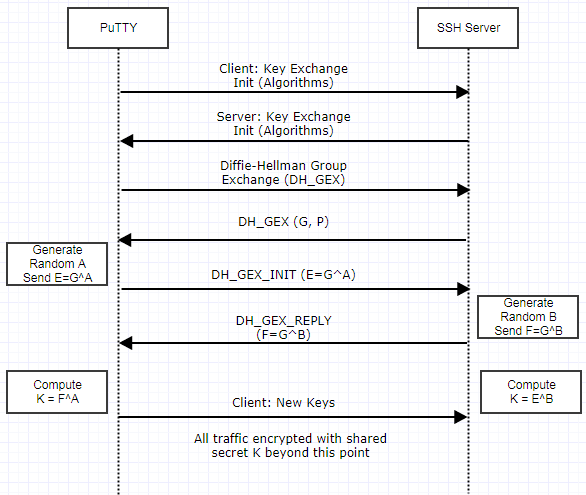
\includegraphics[width=0.72\textwidth]{SSH_DH_KEX.png}
\end{figure}
\section{Public Key Authentication}
A SSH server authenticates a user using either a password or a public key mechanism. When using public key authentication, the possession of a private key serves as authentication \cite{rfc4252}. The SSH client creates a signature using the user's private key. The server check whether public key is a valid authentication mechanism for the user and that the signature verifies. If both the conditions hold the access is granted. Fig. 1.2 offers an overview of the process\par
\begin{figure}[ht]
\caption{Public Key Authentication}
\centering
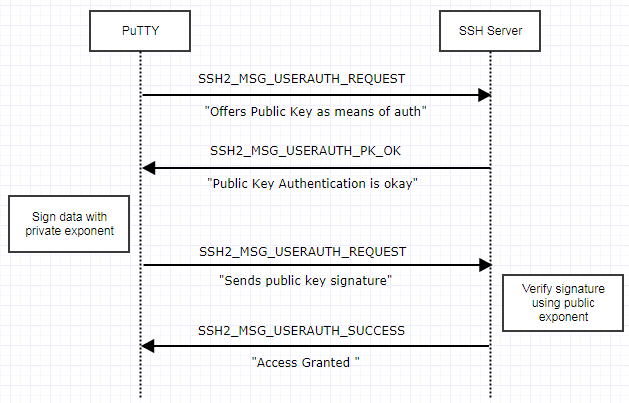
\includegraphics[width=1\textwidth]{SSH_PK_Auth.png}
\end{figure}
\section{Objectives}
\par
Now that we have briefly described the DH Key Exchange and the Public Key Authentication processes of SSH, we move onto outlining the key objectives of the project.\par
As specified earlier our primary objective is to find timing leaks in implementations cryptographic primitives and in that regard we look closely at both the DH Key Exchange and Public Key Authentication portions of the source code. Within this implementations the sections of particular interest to us is the modular exponentiation operations. Both, the DH Key Exchange - during the computation of \(g^a\ mod\ p\) - and the Public Key Authentication - while creating the signature - use modular exponentiation. Both these processes use cryptographically sensitive data in their respective modular exponentiation and a timing leak in these operations could leak the sensitive data. Analysis of these processes is described in chapters 4 and 5.\par

Cryptographic primitives often require a random number generator that generates a random stream of bits. To ensure safety of sensitive data it is critical that this stream of bits be strictly random. To this end our next objective is to analyze and review the code responsible for randomness (a.k.a noise) generation. Additionally to test the statistical properties of the random numbers, we subject them to a variety of test suits. Randomness generation analysis is described in chapter 6\par
In line with our goal of a security audit of the entire software our next objective concerns performing an exhaustive analysis of all invocations of the modular exponentiation operation. This analysis aims to confirm that the data passed to each invocation is safe from tampering by an attacker. By manipulating data to such invocations information about sensitive data could be possibly leaked. Chapter 7 comprises of this analysis.\par
Lastly we analyze and review the implementation of some of the legacy protocols that PuTTY supports. Chapter 8 provides the details of this analysis.\par
\section{Environment Setup}
This section is supposed to acquaint the reader with the setup used for testing and measurements. We describe the audit process and methodology in the next chapter.\par

The source code of PuTTY was downloaded from the PuTTY homepage \cite{putty} and compiled on Windows 7 OS using Microsoft Visual Studio 2015. It provides solutions for all PuTTY projects including those mentioned in section "SSH and PuTTY". Compiling a solution for a project renders an executable. For debugging and flow control analysis, PuTTY was run in debug mode in Visual Studio. For automated measurements a Plink executable with custom additions to code was created. This executable was then invoked from a Java program for multiple measurements \footnote{Refer Appendix A: "Automated Measurements"}. For both debugging and automated measurements a Bitvise SSH Server running on the same host, was used as a server. Alternatively for simulating messages across a network an OpenSSH server running on a Raspberry Pi was used \footnote{Refer Appendix B: "Software and Tools"}.
\chapter{Methodology}
\section{Overview}
The security audit involved analyzing different aspects of the software. To accomplish these analyses several different methodologies were adopted. This chapter briefly explains each one of them.
\section{Code Review}
To perform each analysis, to either rule out the possibility of an attack or to accept it and then attempt to carry out the corresponding attack a deep understanding of the code was required in terms of control flow and data manipulation. As a result code review played a critical role in each of the analysis.
\section{Custom Code}
Specific portions of code were amended to include custom code to make precise timing measurements, manipulate, test and log data values, run desired sections repeatitively etc.
\section{Literature Review}
A review of published literature related to Timing Attacks, Attacks on Diffie-Hellman and RSA/DSA signing provided a sense of possible exploits and attack vectors. Consequently this informed what to look for in a code review. In case of Randomness of Noise Generation check published papers were used to know relevant test suites to use.
\section{Randomness Test Suites}
In addition to the review of the random generation code, generated stream of bits were subjected to a battery of tests from standard test suites.
\chapter{Diffie-Hellman Key Exchange Analysis}
\section{Overview}
In this chapter we attempt a timing attack on the modular exponentiation operation involving the secret exponent for the client within the DH Key Exchange protocol.
\section{Timing Attack on Diffie-Hellman}
In a DH Key Exchange between a client and a server that culminates in a shared secret between the two parties, both the client and the server are required to perform a modular exponentiation operation individually with a secret exponent. This modular exponentiation operation is vulnerable to timing attacks and an attacker may be able to find the secret exponent by carefully measuring the timing required to perform operation \cite{kocher96}.\par
We explored the possibility of this attack being carried out on the DH modular exponentiation implementation within PuTTY by reviewing the relevant code sections. Instead of using the same exponent in each invocation of the Key Exchange, a new random exponent, is generated every time. If this is so, the attack does not work \cite{kocher96}.
\section{Attack on Short Exponents in DH}
In \cite{oorschot96} the authors present a technique that can be used to recover short exponents (160-bit exponents with 1024-bit primes). To explore the possibility of this attack, we analyzed the length of the exponents used by PuTTY in its implementation. The bit-length of the exponent is dependent on the DH group in use. For DH Group 1 with 1024-bit primes, which has the lowest bit-lengths, the length of the exponent is 384 bits. For DH Group Exchange, which is the default when DH is used, wherein the client specifies to the server a minimum, a maximum and a preferred length of bits for the prime, the exponent is 544 bits. So even the shortest exponent supported by PuTTY is sufficiently long. These exponents together with safe primes, which SSH mandates, precludes the above attack.
\chapter{Public Key Authentication Analysis}
\section{Overview}
In this chapter analyze if we are able to exploit any timing attacks within the public key signing process employed to authenticate the user using public key. The intent is to be able to reveal the user's private key.
\section{Public Key Authentication Process}
As mentioned in section 1.4 "Public Key Authentication", in public key authentication the possession of a private key serves as the authentication for the user. In this section we explain the process in detail and then look at the part we are most interested in i.e. the signing with the private key.\par
\clearpage
\begin{figure}[ht]
\caption{Exchange of messages during Public Key Authentication}
\centering
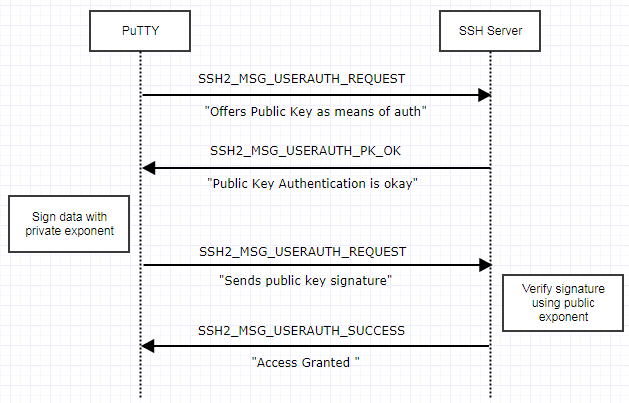
\includegraphics[width=1\textwidth]{SSH_PK_Auth.png}
\end{figure}
The image above provides an overview of the process. The client requests the server to be allowed to use public key as an authentication mechanism. The server responds positively if the user may be allowed to use public key or negatively otherwise. On receiving a positive response the client proceeds to generate and send a signature to the server which is then verified by the server and depending on whether the verification succeeds the server grants access to the user.\par
In the procedure explained above we focus our attention on the operation that generates a signature using the user's private key. The signature is generated over a set of data that includes - the session identifier, hex code identifying the request,user name, service name, the string \textit{public key}, a boolean value \textit{TRUE} identifying that this message contains the actual signature, public key algorithm name and the public key to be used for authentication. To be precise the signature is actually generated over a hash of the above values.

\section{RSA Blinding}
To explore the possibility of a timing attack on the public key signing operation we review the relevant code sections. The file \textit{sshrsa.c} deals with the implementation of the RSA protocol and the public key signing operation is incorporated within the function \textit{rsa2\_sign}. Reviewing the code in this function we observe that PuTTY employs RSA Blinding during the exponentiation to prevent an attacker to be able to draw any correlation between the timing of the operation and the exponent used. Remember the exponent used is the private key (the private exponent of the RSA key). This essentially safeguards against the possibility of a timing  attack. The next paragraph discusses the implementation of the blinding process and how it protects against the attack.\par
We explain how RSA blinding is implemented and how it protects against a timing attack. Let's assume \(x\) is the base or the hash value of data to be signed, \(d\) is the private exponent of the key and \(p\) the modulus. The signature is computed thus - signature \(s\ =\ x^d\ mod\ p\). When this operation is performed by itself minor timing differences in the operation shall reveal the private exponent of the key. We generate a random, say \(y\) and instead of computing  \(x^d\ mod\ p\) we compute \((x*y)^d\ mod\ p\). Note that, \((x*y)^d\ mod\ p\) = (\(x^d\ mod\ p\)) * (\(y^d\ mod\ p\)). Hence, we instead compute the signature thus \(s\ =\ ((x*y)^d\ mod\ p\))/(\(y^d\ mod\ p\)). The benefit this has is that because the attacker has no knowledge of either \(x\) or \(y\) (y is generated randomly using sound randomness), he is unable to correlate the timing of the operation with the value of \(x\) which precludes the timing attack. Please note there have been attacks developed quite recently that can still work even if the software employs RSA blinding. These attacks are termed as the "Cross corelation Attack". Please refer section 9.4 "Cross-corelation Attack" \cite{praveen} of chapter 9 "Further Work".
\section{Random Generation for Blinding}
The random number (\(y\) in above), does not come from the Random Pool maintained as a main source of randomness by PuTTY. Instead the random for the blinding process is generated by hashing different values with the private key.\par
The process begins by choosing a number of the length of the modulus, the position of the top most set bit is found and then randomly setting bits downwards from that bit. Then PuTTY proceeds to hash different things with initial value, lastly the private exponent of the key is hashed with it.\par
The random is chosen uniformly from the range 2-modulus-1. If the random to be chosen is greater than the modulus then a new random computed instead of just reducing the random computed to mod \(n\), to avoid any Bleichenbacher-like attacks making use of the uneven distribution within the said range that would arise from just reducing the number mod \(n\).
\section{An Artificial Attack}
We seek to know whether a timing attack is possible on the signing operation even without the blinding employed. To explore this, we first amend the source code to completely strip off the blinding. In addition to stripping off the blinding code, we also comment out the code for the random generation. In effect we are reverting the code back to performing the simple computation for the signature \(s\ =\ x^d\ mod\ p\).\par
We explore the possibility of applying the attack from \cite{brumley} on the public key signing process after removal of the blinding code. The paper discusses remote attacks on RSA decryption in OpenSSL\footnote{\url{https://www.openssl.org/}}. Decryption is performed by the private exponent of the key as is the signing (our case). PuTTY, like OpenSSL, uses Chinese Remainder Theorem (CRT) to perform the exponentiation for the signing process. Using CRT the exponentiation \(s\ =\ x^d\ mod\ p\) is computed in two steps, first evaluate \(s_1\ =\ x^\{d_1\} \ mod\ p_1\) and \(s_2\ =\ x^\{d_2\} \ mod\ p_2\) (Here, \(p\ =\ p_1\ *\ p_2\) and \(d_1\ and\ d_2\) are pre-computed from \(d\)), second to combine \(s_1\) and \(s_2\) using CRT to get \(s\). A timing attack can expose the factors \(p_1\) and \(p_2\). Revealing the factors effectively reveals the private exponent \(d\) (\(d\ =\ e^\{-1\}\ mod\ (\{p_1\}\ -\ 1 )\ (\{p_2\}\ -\ 1)\) , \(e\) is the public exponent of the key). \par
The authors in \cite{brumley} mention two different sources of timing differences originating in the modular exponentiation process. The first difference in timing arises from the use of Karatsuba or ordinary multiplication for multiplication in the exponentiation operation. Karatsuba being faster runs in shorter time. The second difference originates from what is called as an "Extra Reduction" at the end of Montgomery reduction. Montgomery reduction transforms a reduction modulo \(p\) (the modulus) into a reduction modulo some power of 2 which can be efficiently implemented as a series of operations in hardware. At the end of the reduction the final result is checked to see if it is greater than the modulus \(p\). If it is than the result is reduced modulo \(p\) to ensure the result is in the range [\(0\ -\ q\)). This step is named as the "Extra Reduction" and causes timing differences in different inputs. The probability that an Extra Reduction will be required increases as the base \(x\) approaches the modulus \(p\) from below, at values of \(x\) that are multiples of \(p\) the probability drops sharply to zero. If the timing measurements are recorded onto a graph the increasing time for the operation  as \(x\) approaches \(p\) from below followed by sharp drops at \(x\) equal multiples of \(p\), form peaks on the graph that help us make estimations at the values of \(p\). We can then by making educated manipulations to the value of \(x\) figure bits of \(p\).
\section{PuTTY's Exponentiation Implementation}
To explore the possibility of carrying out this attack on PuTTY's implementation, we begin by reviewing implementation of the exponentiation operation. We investigate whether the two above mentioned sources of timing differences do indeed exist in PuTTY's implementation. If they do we can proceed to perform a similar attack from \cite{brumley}.\par
PuTTY implements both the Karatsuba and the ordinary multiplication algorithm for performing the multiplications resulting from the exponentiation. Though it exercises a  threshold on the size of the modulus of the exponentiation to decide whether or not Karatsuba should be used. This threshold defined in the file \textit{sshbn.c} is 50 words (50 * 32 = 1600 bits on 32-bit platforms and 3200 bits on 64-bit platforms). If the modulus is smaller than 50 words ordinary multiplication algorithm is used. With CRT in use this threshold restriction applies not to the original modulus but to \(p_1\) and \(p_2\), the moduli that apply to the two split exponentiations performed by CRT, remember \(p\) = \(p_1\) * \(p_2\). Since the most common bit-length for an RSA key modulus is 2048, the factors \(p_1\) and \(p_2\) are typically half the size or 1024 bits in length. Even with a 3072-bit modulus for RSA, the factors are typically 1536 bits in length. As a result PuTTY almost always ends up using only the ordinary multiplication algorithm and almost never using Karatsuba. This results in one of the sources of timing differences as identified in \cite{brumley} not being so in PuTTY.\par

\chapter{Randomness Generation Analysis}
\section{Overview}
In this chapter we analyze the randomness generation process in PuTTY. The aim is to find the sources for the randomness and how they are used. We also subject the random numbers generated through some standard test suites and interpret the results here.
\section{Randomness Generation Process Overview}
PuTTY maintains a pool of size 1200 bytes of random generated data, from which it hands out bytes of data to processes that request it. This pool of data is filled at start-up from noise generated from various sources such process listings, local-time, random files on search paths and other environmental noise. A seed from a seed file that is maintained by PuTTY in the Windows Registry is also used. This process is called "heavy noise generation" and occurs only once in one invocation cycle.\par
This generated random data then undergoes a process what PuTTY calls "Random Stir". This random stirring involves two passes of SHA (Secure Hash Algorithm) Transformation where SHA is operated in CFB (Counter Feedback) mode and the output is repeatedly fed back to the SHA digest.\par
Random noise is generated in the background every 5 minutes and added to a buffer known as "incoming buffer". When this buffer gets full, the contents are added to another hold area called simply as "incoming" where it will be held to be used for "stirring" the pool when required.\par
Data from this random pool is handed out to a requesting entity such as PuTTY's implementations of cryptographic primitives. PuTTY maintains a pointer to the pool and advances this pointer as it hands out random data until the pointer reaches the end of the pool at which point the pool is stirred again using noise generated so far from the environment in the incoming buffer and the pointer is reset to its starting position.\par
\begin{figure}[ht]
\caption{Randomness Generation Process in PuTTY}
\centering
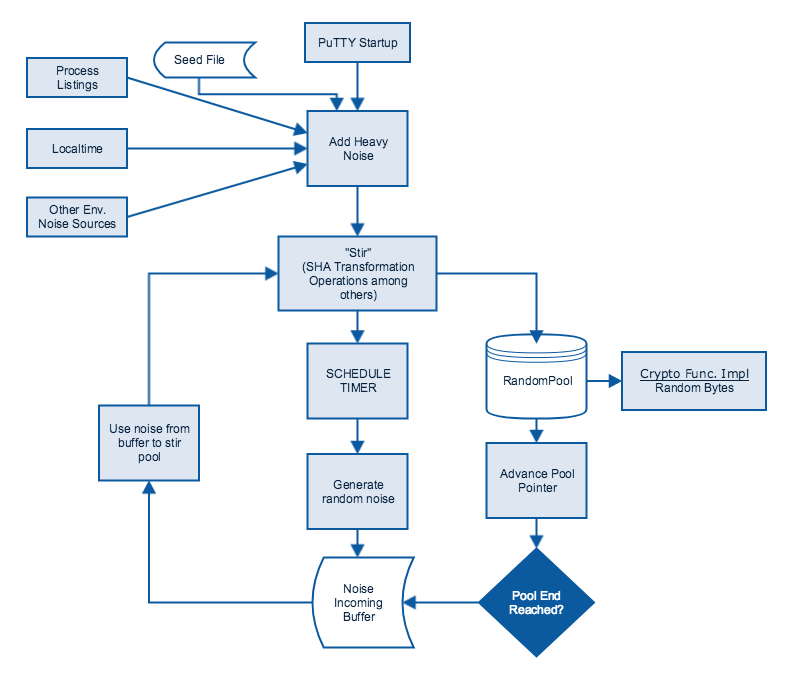
\includegraphics[width=1\textwidth]{NG.png}
\end{figure}
\section{Random Generator Tests}

\chapter{Modular Exponentiation Analysis}
\section{Overview}
This chapter analyzes whether an attacker, by being able to manipulate arguments passed to a modular exponentiation invocation carry out timing attacks to reveal cryptographically sensitive data values.
\section{Modular Exponentiation Review}
PuTTY implements a modular exponentiation operation that is invoked by implementations of primitives such as RSA, DSS, ECC and DH. We exhaustively review each of these invocations to study and analyze the source of the arguments passed to the operation with the aim to discover whether an attacker would be able to tamper with the arguments. The ability to manipulate data arguments to the modular exponentiation algorithm would give an attacker the ability to measure the slight timing differences in the runtime of the operation as a result of variable arguments.\par
The modular exponentiation operation in PuTTY is called \textit{modpow} and is invoked with three arguments - base, exponent and the modulus. We list each invocation and analyze it here.\par
\clearpage
\begin{enumerate}
    \item \textbf {Diffie-Hellman Implementation}
    In DH the \textit{modpow} operation is invoked twice. Once for the computation of \(e\ =\ g^a\ mod\ p\) and once for computing the shared secret \(K\ =\ f^a\ mod\ p\). While both invocations include arguments that are sourced over the network - \(g\) and \(p\) in the first and \(f\) in the second invocation - it does not make sense for an attacker to tamper these. An attacker in this case, would be acting as a man-in-the-middle between the client and the server and would have a DH shared key negotiated both with the client and the server individually. We can conclude that both these invocations are safe against possible tampering from an attacker.
    \item \textbf {DSA (Digital Signature Algoritm) Implementation}: 
    In DSA implementation the \textit{modpow} operation is invoked a total of four times - twice in the DSA signature verification - computing \(g^{u_1} \ mod \ p \) and \(y^{u_2}\ mod \ p\), once in DSA public key creation and once in DSA signing - computing \(g^k \ mod \ p\).\par
        \begin{enumerate}
        \item \textbf \underline{DSA Signature Verification}    \begin{itemize}
            \item {\(g^{u_1} \ mod \ p \)}: Both \(g\) and \(p\) come from the DSA as negotiated parameters. \(u_1\) is computed internally from other values.
            \item {\(y^{u_2} \ mod \ p \)}: \(y\ = \ g^x\ mod \ p\) and \(p\) comes from DSA as negotiated parameter. \(u_2\) is computed internally from other values.
         \end{itemize}
        The attacker cannot manipulate \textit{modpow} arguments to exploit any timing attacks.
        \item \textbf \underline{DSA Public Key Creation}
        \begin{itemize}
        \item
        The \textit{modpow} operation is called within the public key creation operation to verify \(y \ =\ g^x \ mod \ p\). Parameters \(g\) and \(p\) are DSS parameters and \(x\) is the secret exponent generated randomly internally. The attacker cannot manipulate any of these arguments to his benefit.
        \end{itemize}
        \item{DSA Signing}
        \begin{itemize}
        \item
        Used to compute \(g^k \ mod \ p\) where \(g\) and \(p\) are DSA parameters and \(k\) is generated randomly. Since none of the parameters come from external sources the attacker cannot manipulate them.
        \end{itemize}
        \end{enumerate}
    \item \textbf{ECC (Elliptic Curve Cryptography) Implementation}:
        In the ECC implementation \textit{modpow} is used thrice, once in point verification and twice in for Edward curve.
        \begin{enumerate}
            \item {Point Verification}:
            Computation of \(x^3\ mod\ p\). Parameters are either ECC parameters or are computed internally elsewhere within the calling operation.
            \item{Edwards Curve}:
            Both invocations for the Edwards Curve are heavily dependent on arguments that are computed elsewhere in the calling operation. No arguments have external sources.
        \end{enumerate}
        The attacker does not have an option to tamper with arguments to attack the \textit{modpow} operation to reveal any sensitive values.
    \item \textbf{RSA Implementation}: For RSA implementation the \textit{modpow} operation is invoked a total of five times - once for encryption with the RSA public key, twice from within CRT (Chinese Remainder Theorem) optimization to compute the result modulo the two modulus \(p\) and \(q\), once for verifying a RSA host key for the server and lastly for encryption in RSA Key Exchange.
        \begin{enumerate}
            \item{RSA Encrypt}: The base is the SSH session-key, stored internally, the exponent is the key's public exponent, the modulus is the key's modulus (not secret). Since the public key is assumed to be installed safely prior to this operation, we conclude that the attacker cannot manipulate arguments for to his benefit.
            \item{CRT Optimization}: In both the modular exponentiation calls all the arguments are sourced either from within the calling operation itself or from a calling function one level higher, but since the arguments aren't influenced by external values, the attacker as no possibility of being able to manipulate the arguments.
            \item{Signature Verification}: This invocation of \textit{modpow} is within the RSA host key verification. Even if the attacker can manipulate the parameters to the operation such as the signature it won't be of any benefit to him as the only data that can be revealed (even if) is the signature that he himself sent us, the other parameters such as the key exponent and the modulus are public.
            \item{RSA Key Exchange Encrypt}: All data arguments have source internal to PuTTY, so the attacker cannot tamper with the data in any way.
         \end{enumerate}   
\end{enumerate}    
\chapter{Legacy Protocols Analysis}
\section{Overview}
In this chapter we examine legacy protocols supported by PuTTY with the aim to find any possible vulnerabilities in their implementation.
\section{Motivation}
Protocols that are old and aren't mainstream anymore may have vulnerabilities that are overlooked because the portion of code dealing with them is rarely used, or because such code would not be tested nearly as heavily as the code dealing with default, most commonly used protocols, or simply because a new attack makes the code vulnerable. Such protocols maye be supported just because of compatibility issues with genuine old servers. Even though these protocols aren't default, this won't stop an attacker with a malicious SSH server to make them be chosen by downgrading the list of supported protocols on his malicious server. Once the protocol is in use he can exploit any existing vulnerability.
\clearpage
\section{Analysis of Diffie-Hellman Group 1}
For Key Exchange PuTTY supports DH Group 1 which is a very weak DH group of 1024-bits. We must note that PuTTY does warn the user against selecting this protocol as is evident from the image below.
\begin{figure}[ht]
\caption{Warning against use of weak DH Group for Key Exchange}
\centering
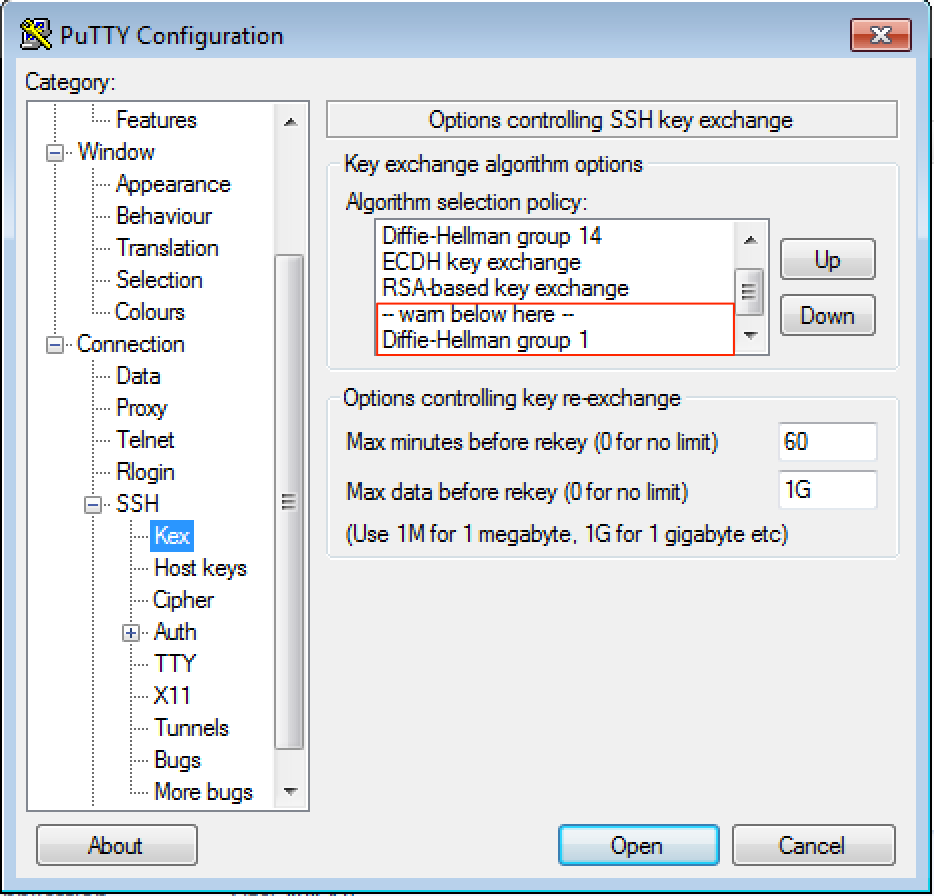
\includegraphics[width=1\textwidth]{legacy.png}
\end{figure}
We traced the control flow for this protocol and reviewed the code in use. Having a 1024-bit group, it is vulnerable against nation-states adversaries against the LogJam attack \cite{adrian}. This, understandably is not a vulnerability in PuTTY. The secret exponent (client's secret) under this group is significantly shorter (384-bits) than the typical value (544-bits). Upon inspection though we find that the code segment used is the same as that for higher stronger groups. Only difference apparently is that DH is initialized with smaller values for the prime \(p\) which affects \(q\) which in turn affects the secret exponent \(x\) which is as mentioned above significantly shorter. \par
Since the instruction set essentially remains the same as that for any DH group, this group is not exposed to any vulnerabilities just on account of being a legacy, rarely used protocol. It should exibit the same cryptographic security properties as any DH implementation. Thus we can conclude that the support of weaker protocols for the Key Exchange does not make PuTTY insecure by itself.
\chapter{Conclusions}
\chapter{Further Work}
\section{Overview}
This chapter provides overview of work that can be undertaken as an extension of this project. Carrying out tasks listed here shall make for a broader security audit of the software and weren't included in this project due to time restrictions.
\section{Cache-based Timing Attacks}
\section{Buffer Overflows}
\begin{appendices}
\chapter{Automated Measurements}
\chapter{Software and Tools}
\end{appendices}
\begin{thebibliography}{9}
\bibitem{putty}
PuTTY
\url{https://www.chiark.greenend.org.uk/~sgtatham/putty/}
\bibitem{rfc4251}
RFC 4251, The Secure Shell (SSH) Protocol Architecture,\\
\url{https://tools.ietf.org/html/rfc4251}
\bibitem{rfc4252}
RFC 4252, The Secure Shell (SSH) Authentication Protocol,\\  \url{https://tools.ietf.org/html/rfc4252}
\bibitem{rfc4253}
RFC 4253, The Secure Shell (SSH) Transport Layer Protocol,\\ \url{https://tools.ietf.org/html/rfc4253}
\bibitem{rfc4254}
RFC 4254, The Secure Shell (SSH) Connection Protocol,\\ \url{https://tools.ietf.org/html/rfc4254}
\bibitem{randeval}
Randomness Evaluation Framework of Cryptographic Algorithms,\\
\url{http://www.academia.edu/9902264/Randomness_Evaluation_Framework_of_Cryptographic_Algorithms}
\bibitem{kocher96}
Paul C. Kocher, Timing Attacks on Implementations of Diffie-Hellman, RSA, DSS  and Other Systems. Annual International Cryptology Conference, Advances in Cryptology, CRYPTO' 96, pp 104-113
\bibitem{oorschot96}
On Diffie-Hellman Key Agreement with Short Exponents, Paul C. van Oorschot, Michael J. Wiener, International Conference on the Theory and Applications of Cryptographic Techniques, Advances in Cryptology — \\EUROCRYPT '96, pp 332-343
\bibitem{praveen}
Attacking OpenSSL using Side-channel Attacks: the RSA case study, Praveen Kumar Vadnala,Lukasz Chmielewski
\bibitem{brumley}
Remote Timing Attacks are Practical, David Brumley, Dan Boneh, Computer Networks, Volume 48, Issue 5, 5 August 2005, Pages 701-716
\bibitem{adrian}
Imperfect Forward Secrecy: How Diffie-Hellman Fails in Practice, David Adrain et al.CCS '15, Proceedings of the 22nd ACM SIGSAC Conference on Computer and Communications Security
pp 5-17
\end{thebibliography}
\listoffigures
\end{document}
